%
% chapter2.tex
%

\chapter{Smart NICs - ein Überblick}
\label{cha:background}
In diesem Kapitel wird ein allgemeiner Überblick über die Architektur einer intelligenten Netzwerkkarte gegeben.

\section{Begriffserklärung}
Der Begriff \textbf{Smart Network Interface Card} (Smart NIC) ist wie allzu oft in der Computerwissenschaft mit einer Menge von Definitionen versehen. Grundsätzlich beschreibt eine Smart NIC eine Hardwareeinheit, deren Funktion die Netzwerkfähigkeit eines Rechners beschreibt. Dabei unterscheidet sie sich von den klassischen Netzwerkkarten in der Hinsicht, dass wir als Anwender beziehungsweise Entwickler Anwendungen schreiben können, die das Verhalten der Karte beeinflussen. Dabei ist nicht fest definiert, welche Funktionen gebaut werden oder überhaupt, in welchem Umfang programmiert werden kann. Nicht zuletzt ist das immerwährende Aufkommen des Begriffs Smart* dafür verantwortlich, dass sicherlich auch aus Marketinggründen ein entsprechender Name gewählt wurde. Allgemein ist eine Smart NIC eine Netzwerkkarte, die es erlaubt, Anwendungen zu erstellen, die ihr eigenes Verhalten derart verändern kann, dass Funktionen, die sonst innerhalb eines Netzwerkstapels übernommen werden würden, nun auf der Netzwerkkarte selbst ausgeführt werden können. \cite{smartnicsComproSurvey}

\section{Aufbau und Funktionsweise}
Smart NICs verwenden unterschiedliche Hardwarearchitekturen, um eine Hardwarebeschleunigung zu realisieren. Allgemein gab es sogar in den 90er- und frühen 2000er-Jahren Smart NICs, die lediglich oder größtenteils klassische Prozessorarchitekturen wie RISC oder x86 verwendeten. Mit Anbruch des neuen Jahrtausends zogen jedoch immer mehr FPGA- und ASIC-basierte Architekturen in die Rechenzentren ein. \cite{towardsSmartNICCluster}
\begin{figure}
    \centering
    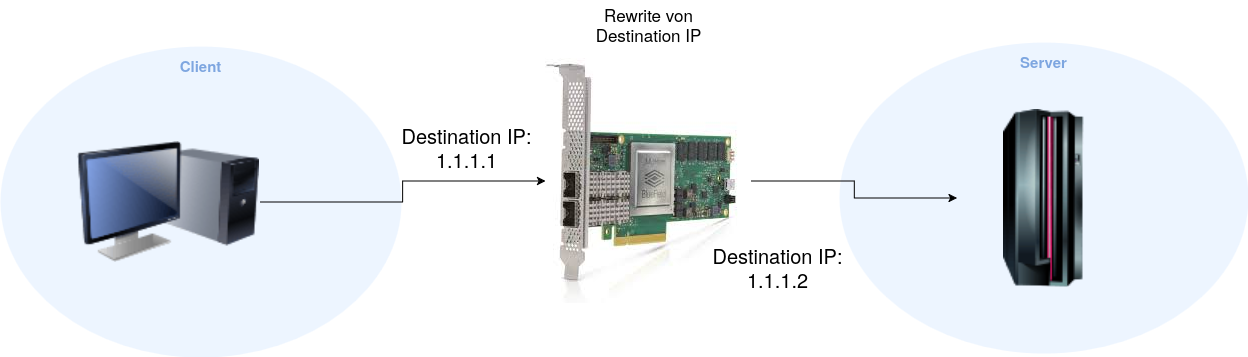
\includegraphics[width=1\linewidth]{images/GrundaufbauSmartNIC.drawio.png}
    \caption{Einfaches Ändern einer IP-Adresse im Paket}
    \label{fig:enter-label}
\end{figure}
Das steigende Interesse an der SmartNIC Architektur ist nicht zuletzt durch den abflachenden Leistungsgewinn durch Generationsfortschritte in der Prozessorindustrie befeuert worden. Mittlerweile gilt das Moorsche Gesetz als beendet und ein Großteil der Computerkommunikation heutzutage ist ohnehin Netzwerkverkehr. \cite{endofmoore} Meistens werden dazu TCP- und UDP-Pakete verwendet. Werden diese Pakete auf Prozessoren verarbeitet, sind die entsprechenden Kosten nicht nur hardware- sondern auch energieseitig sehr hoch. Zuletzt hat nun auch der Aufschwung der modernen Softwarearchitekturen für einen explosionsartigen Anstieg in Netzwerkverkehr gesorgt. Wurden vor zwanzig Jahren Anwendungen noch so entwickelt, dass möglichst wenig Kommunikation über ein Netzwerk läuft, wird in heutigen Systemen stark und immer mehr auf eine Microservice-basierte Architektur gesetzt. \cite{microservices} Dabei wird eine komplexe Applikation in verschiedene Bereiche unterteilt, die daraufhin mittels HTTP-angebundenen Interfaces miteinander kommunizieren. Grund dafür ist die Idee der vereinfachten Wartbarkeit von kleinteiligen Applikationen.
Zu Beginn der Entwicklung besagter Hardware war zunächst grundsätzlich die Idee, die programmierbare Funktionalität auf dem Switch, also dem Anbindungspunkt des Rechenzentrums, umzusetzen. Allerdings steigt mit der Anzahl der Knoten im Teil hinter dem Switch auch die benötigte Rechenkapazität des Switches. \cite{smartswitches} Daher hat sich ein eher dezentraler Ansatz entwickelt, bei dem in dem Server selbst eine Karte integriert ist, auf der sich ein zusätzlicher Rechner befindet. Dabei ist die Verbindung zugunsten der größten Kompatibilität meist mittels PCI-Express umgesetzt. In der Abbildung 2.1 ist ein grundsätzliches Diagramm eines hier abstrahierten Datenpakets dargestellt. Der Client schickt ein Paket mit einer bestimmten Ziel-IP-Adresse los und zu einem gewissen Zeitpunkt erreicht das Paket die Smart NIC. Diese wendet daraufhin eine Aktion an. In diesem Fall wird die Ziel-IP-Adresse geändert und zurück in das Netzwerk geleitet. Dadurch bekommt nun ein anderer Server das Paket. Hierbei ist interessant, dass die Umleitung dem Client verborgen bleibt. Im Prinzip handelt es sich also bei dem gezeigten Beispiel um einen primitiven L3-Proxy.
\subsection{Hardwareaufbau}
SmartNICs sind in aller Regel im Grunde völlig eigenständige Systeme mit Prozessoreinheit, Arbeitsspeicher und teilweise sogar eigenständiger Netzwerkein- und -ausgabe über einen separaten Hardwareport. Die Idee dabei ist es, ein System zu schaffen, auf dem eigenständig Applikationen ausgeführt, aber auch Dienste wie Docker oder Kubernetes angewendet werden können. So wird auch die Verbindung zur Entwicklung über etwaige Dienste wie SSH hergestellt. Allerdings bieten auch einige Hersteller eigenständige Lösungen an, welche in aller Regel mittels \textbf{Application Programming Interfaces} kurz APIs zur Verfügung gestellt werden. Hauptgrund sind allerdings, wie so oft in solch hochkritischen Systemen, Sicherheitsbedenken. Eine vollständig getrennte Einheit unterstützt in diesem Sinne das Konzept der Zero-Trust-Paradigmen. Dabei wird angenommen, dass allen Kommunikationspartnern sowie allen Beteiligten in einem System nicht zu trauen ist. Eine SmartNIC kann somit völlig autark in einem Netzwerk fungieren, ohne dass das Hostsystem selbst den Aufbau des Netzwerks oder dessen Funktionsweise kennt. \cite{whatyouneedtoknowaboutsnics} Die besonders im Kontext der Netzwerkverarbeitung relevanten Hardwareeinheiten werden mittels fest verarbeiteter Hardwareinterfaces angesprochen. Dabei werden meist die vorliegenden PCI-Lanes als Hochgeschwindigkeitsverbindung genutzt. Und genau hier wird auch einer der größten Unterscheidungspunkte zwischen der klassischen Netzwerkpaket verarbeitenden Hardware und den modernen SmartNICs deutlich. Die meisten anderen Netzwerkadapter verwenden Mikrocontroller, um eine Konfigurierbarkeit zu gewährleisten. Die Kommunikation zwischen den Mikrocontrollern und den tatsächlichen Hardwarebeschleunigern erfolgt daraufhin meist mittels serieller Schnittstellen statt. Dabei ist natürlich das Hauptunterscheidungsmerkmal der Prozessortakt. Klassische SmartNIC \textbf{Systems on a Chip} kurz SoC verwenden Prozessoren mit mehreren Kernen, die in einem ähnlichen Bereich getaktet sind wie etablierte Server- oder Desktopchips. Dabei ist die Leistung vor allem relevant, da auch klassische Berechnungen auf den Kernen ausgeführt werden sollen. Bei den kleineren, schwächeren Mikrocontroller-Prozessoren liegen die Taktraten größtenteils klar unter 1 GHz. Diese werden allerdings auch eben nur für Konfiguration und Management verwendet und übernehmen keine direkte Aufgabe, die an der Paketverwaltung beteiligt ist. Zusammenfassend lässt sich also eine grobe Unterteilung vornehmen, bei der sich die SoC-Varianten der SmartNICs klar von denen unterscheiden, die diskrete Hardwareeinheiten für den jeweiligen Verwendungszweck besitzen.
\subsection{Path Switching}
Über die letzten Jahre haben sich unter diversen anderen architektonischen Ansätzen zwei etabliert, welche für den Kontext dieser Arbeit von besonderer Bedeutung sind. Es wird hauptsächlich durch die Switchting-Funktionalität unterschieden. Die zwei entstehende Klassen sind On-Path-Switching und Off-Path-Switching (siehe Abbildung 2.2).
\subsubsection{On-path-SmartNICs}
Bei einer On-Path-SmartNIC verhält sich die Netzwerkkarte sehr nahe an der Funktionsweise, wie man sie von einer traditionellen Netzwerkkarte erwarten würde. Pakete, die über das Kabel an die Hardware herantreten, werden zunächst von dem entsprechenden Stack der Karte verarbeitet und laufen gezwungenermaßen nicht nur über den Traffic-Manager, sondern insbesondere auch über die Kerne der SmartNIC. \cite{onoffpath} Das heißt zwar, ein nicht unerheblicher Overhead bei der Verarbeitung des Datenverkehrs entsteht im Kernel des Betriebssystems. Es ermöglicht aber eben auch, Modifikationen an besagten Paketen vorzunehmen. Dabei steht vor allem auch die vereinfachte Entwicklung solcher Netzwerkkarten im Vordergrund. Sollte es sich wiederum um eine On-path-SmartNIC handeln, bei der Pakete direkt über den Kernel des Hostrechners verarbeitet werden, stellt sich hierbei das Problem dar, dass es so zu einer Überlastung der Anbindung zwischen SmartNIC und Host kommen kann. Außerdem liegt in solch einem Fall dann ein Großteil der Rechenlast wieder beim Host, womit die eigentliche Funktionalität der SmartNIC stark abnimmt. 
\subsubsection{Off-path-SmartNICs}
Bei Off-Path-SmartNICs handelt es sich hingegen um Geräte, bei denen eine klarere Trennung der Hardwareeinheiten vorgenommen wird. Eben diese Trennung ermöglicht eine Spezialisierung, mit der für bestimmte Anwendungszwecke besondere Hardwarebeschleuniger verbaut werden können. Diese Architektur erlaubt es, einen wesentlich größeren Anwendungsbereich abzudecken, da dadurch eine große Flexibilität für die Verarbeitung von Datenpaketen gewährleistet wird. Wenn ein Paket eintrifft, muss es nicht von einem Prozessorkern der Netzwerkkarte beachtet werden, sondern kann von der speziellen Hardwareeinheit verarbeitet werden. \cite{onoffpath} Dabei werden in aller Regel \textbf{Application Specific Integrated Circuits}, kurz ASICs, verwendet. Die Konfiguration dieser ASICs erfolgt dann meistens mittels Software, die auf dem Prozessor der Netzwerkkarte läuft. Allerdings gibt es dort auch Unterscheidungen, ob die Anwendung zur Konfiguration auf dem Hostsystem, also dem Rechner in dem die SmartNIC eingebaut ist, oder der Karte selbst ausgeführt werden soll. Off-path-SmartNICs verbessern somit die gesamte Architektur, indem sie die Allgemeinen Kerne des Prozessors klar vom kritischen Pfad der Netzwerkpakete trennen und es so verhindern, dass die logische Last, welche mit einer Anwendung einhergehen kann, sich in keinster Weise auf den tatsächlichen Durchsatz der Netzwerkkarte auswirken können.
\begin{figure}
    \centering
    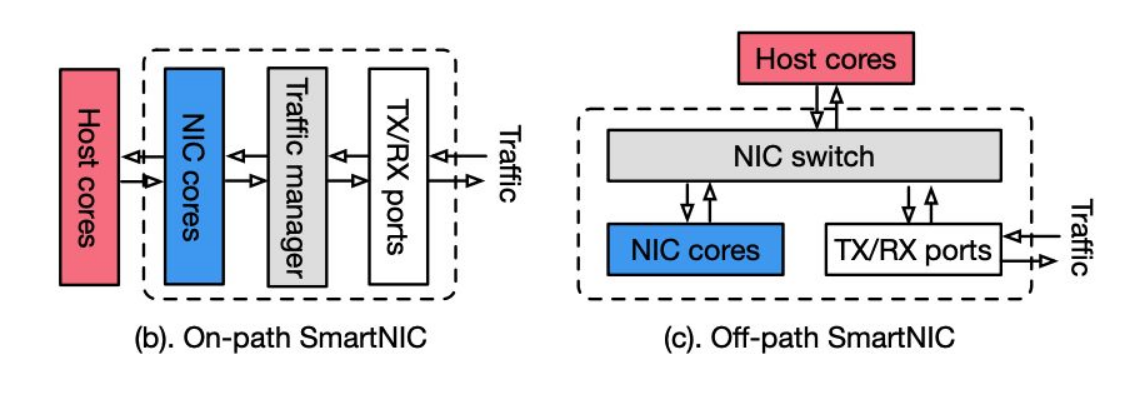
\includegraphics[width=0.9\linewidth]{images/Screenshot 2025-03-16 at 10-41-14 Netdev 0x14 -- Taking Control of your SmartNIC v1.pdf.png}
    \caption{On-Path vs. Off-Path-Switching \cite{onoffpathpic}}
    \label{fig:enter-label}
\end{figure}
\begin{figure}
    \centering
    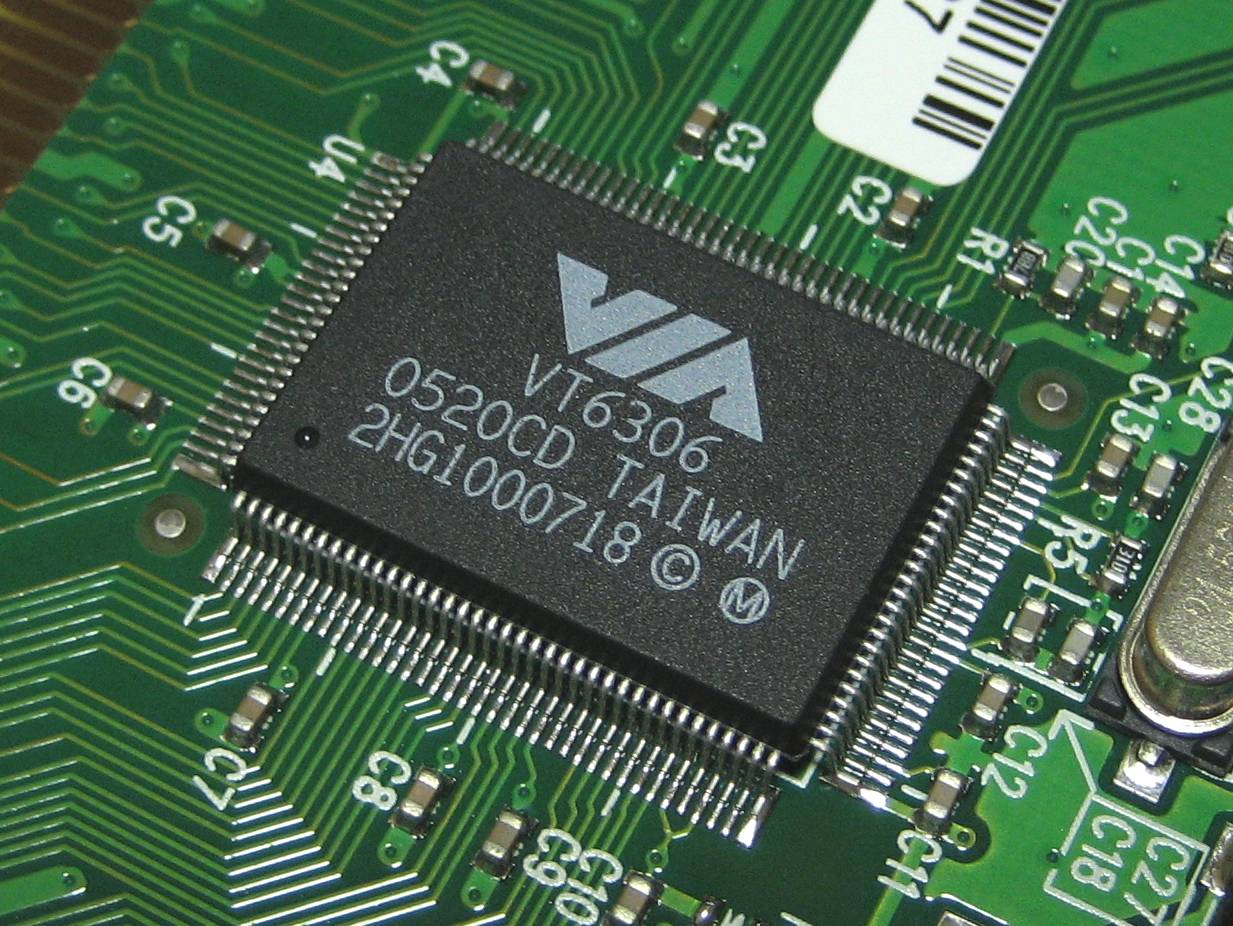
\includegraphics[width=0.5\linewidth]{images/Buffalo_IFC-ILP4_VIA_VT6306.jpg}
    \caption{Firewire ASIC - VIA CT6306 \cite{firewireasic}}
    \label{fig:enter-label}
\end{figure}
\subsection{Application Specific Integrated Circuits}
\begin{figure}
    \centering
    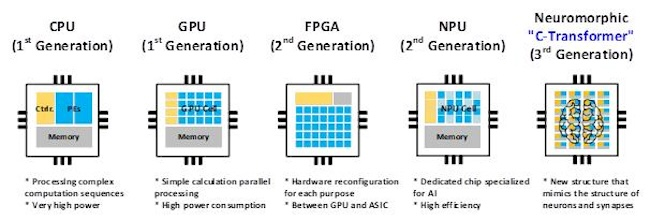
\includegraphics[width=0.8\linewidth]{images/lowpowerasic.png}
    \caption{KAIST LLM Accelerator \cite{kaist}}
    \label{fig:enter-label}
\end{figure}
Application Specific Integrated Circuits (ASICs) sind Hardwareeinheiten, die ein sehr großes Anwendungsgebiet entwickelt haben. So werden sie nicht nur in Netzwerkbeschleunigern verwendet, sondern werden immer dann verwendet, wenn der Zweck der Hardware sich gut beschreiben lässt und somit keine große Varianz an Aufgaben von der entsprechenden Einheit übernommen werden muss. So wird es nämlich den entsprechenden Ingenieuren erlaubt, statt eines allgemeinen Rechners eine hochspezialisierte Einheit zu entwickeln, bei der die Merkmale einer klassischen Prozessorrecheneinheit vernachlässigt werden können. Dadurch ist eine wesentliche Effizienzsteigerung möglich, die es erlaubt, mit wesentlich weniger Energie die gleiche Leistung zu erzielen, wie sonst eine vergleichbare Recheneinheit \cite{asic}. Für rechenintensive Systeme hingegen lässt sich die gesteigerte Effizienz nutzen. Somit kann der allgemeine Durchsatz angehoben werden und es sind Systeme realisierbar, die mit der Anwendung klassischer Rechenwerke erheblich mehr Aufwand bedeuten würden. Zudem erzeugen solche Systeme deutlich mehr Abwärme und würden die Entwicklung somit auch vor ein thermodynamisches Problem stellen. Der Überbegriff ASIC ist nur sehr allgemein und gibt ähnlich wie bei Prozessoren keine Auskunft über die genaue Implementierung. Es gibt viele Architekturen, die für ASICs zur Anwendung kommen, da eben auch die Gebiete weitreichend sind und sich sehr divers unterscheiden. In Abbildung 2.3 ist ein ASIC zu sehen, der die Kommunikation zwischen einem Prozessor und einem sogenannten FireWire-Anschluss eines Endgerätes realisiert. Es muss festgelegt sein, welcher Standard von Geräten mit besagtem Anschluss erwartet wird, um den Prozessor des Hostgerätes mittels eines ASICs zu entlasten.
\newline

Der Zeitgeist in der Computerwissenschaft färbte letztlich außerdem das immens steigende Interesse an Machine Learning ab. Proportional dazu stieg das Interesse an effizienterer Hardware an, da etwaige Lernprozesse extrem energie- und somit kostenaufwendig sind. Es zeigt sich aktuell ein gesteigertes Interesse daran, ASICs zu fertigen, die effiziente hochdimensionale Vektoroperationen umsetzen. Dazu gibt es bereits mehrere Ansätze, mit denen beispielsweise LLM auf einer ASIC-Architektur ausgeführt werden können (siehe Abbildung 2.4). Machine Learning bietet großes Potenzial, Energie mittels ASICs zu sparen, da bisher GPUs und CPUs zum Einsatz kamen, die beide große Energiekosten mit sich bringen. So erlauben ASICs eine extreme Effizienz im Hinblick auf Leistung/Energiekosten.

Abbildung 2.5 zeigt die Leistungsniveaus der unterschiedlichen Architekturen bei einem Bitcoin-Mining-Algorithmus. Im Wesentlichen wird beim Mining etwaiger Kryptowährungen eine Hashsumme berechnet, mit der ein Teil der Blockchain validiert wird. Dabei wird im Falle von Bitcoin ein SHA-256 Hash verwendet. Da es sich dabei um eine sehr allgemeine Berechnung handelt, kann ein guter Vergleich zu vielen anderen Berechnungen gezogen werden. So zeigt Abbildung 2.5, wie sehr in manchen Fällen Algorithmen hinsichtlich ihrer Laufzeit von speziellen Architekturen profitieren können.

\begin{figure}
    \centering
    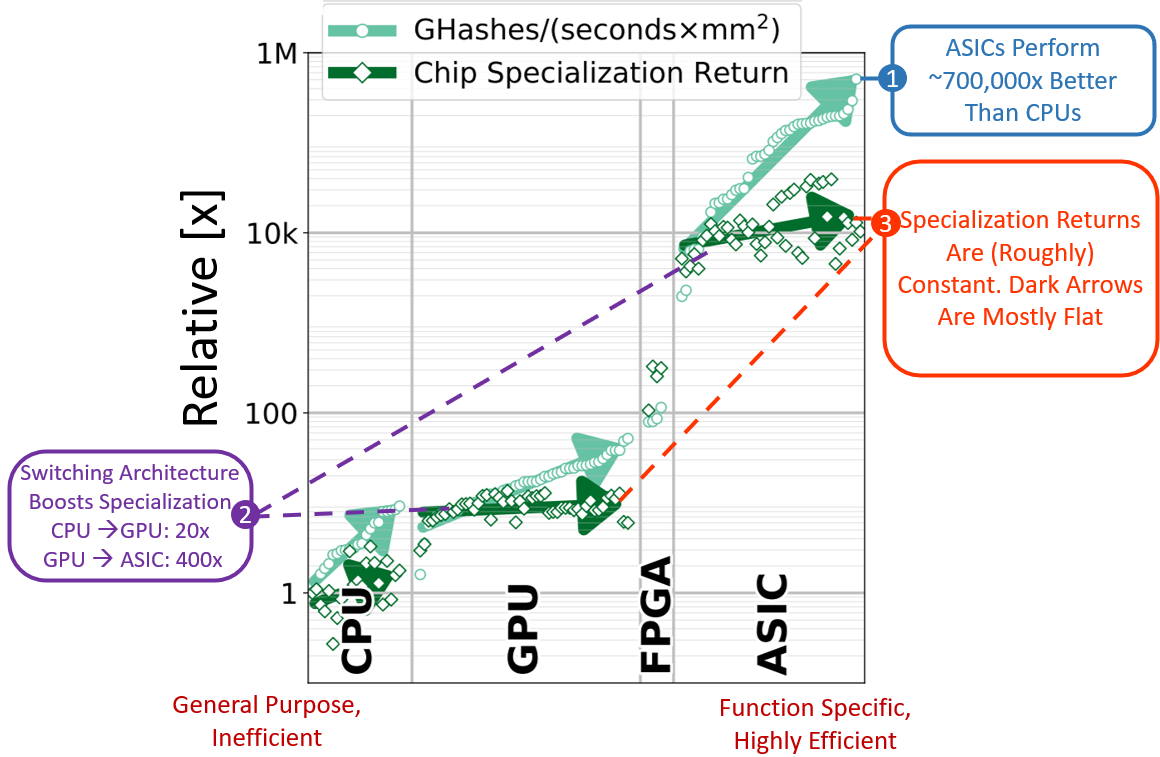
\includegraphics[width=0.7\linewidth]{images/aisic.png}
    \caption{Hardware-Architekturen beim Bitcoin Mininig \cite{bitcoin}}
    \label{fig:enter-label}
\end{figure}
\subsection{Speedup}
Im Allgemeinen werden die Leistungen in eine Metrik gegossen, damit ein objektiver Vergleich vorgenommen werden kann. Dazu entwickelte sich der allgemeine Speedup, der beschrieben wird durch: \cite{speedup}

\begin{equation}
\text{Speedup} = \frac{T_{\text{alt}}}{T_{\text{neu}}}
\end{equation}

Dabei ist:
\begin{itemize}
  \item $T_{\text{alt}}$ die Ausführungszeit vor der Optimierung bzw. der Vergleichshardware
  \item $T_{\text{neu}}$ die Ausführungszeit nach der Optimierung bzw. der Vergleichshardware
\end{itemize}
Um einen Vergleich zwischen den unterschiedlichen Lastverteilungsarchitekturen aufzuzeigen, wird im Folgenden der allgemeine Speedup verwendet.